\documentclass[conference]{IEEEtran}
\usepackage{tabularx}
\usepackage{cite}
\usepackage{graphicx}
\usepackage{float}
\usepackage{hyperref}
\usepackage{amsmath,amssymb}
\DeclareMathOperator*{\argmax}{arg\,max}
\DeclareMathOperator*{\argmin}{arg\,min}
\counterwithout{figure}{subsection}
\usepackage{xcolor}
\usepackage[utf8x]{inputenc}
\counterwithout{table}{section}
% \usepackage{pdfpages}
% \hypersetup{pdfborder=0 0 0}

\begin{document}
\def\refname{\textbf{References}}

\title{Traffic Signal Control Adaptation using Deep Q-Learning with Experience Replay}

\author{
    
    \IEEEauthorblockN{Walid Shaker}
    \IEEEauthorblockA{\textit{Innopolis University}\\
    Innopolis, Russia\\
    w.shaker@innopolis.university}
 
    \and
    
    \IEEEauthorblockN{Siba Issa}
    \IEEEauthorblockA{\textit{Innopolis University}\\
    Innopolis, Russia\\
    s.issa@innopolis.ru}
    
}
\maketitle
\IEEEpeerreviewmaketitle


\begin{abstract}
Traffic congestion is a major area of concern that grab the researchers attention for many years.Traffic congestion can be effectively controlled by using traffic signals that adapt to real-world traffic scenarios. In this paper, we discuss using deep Q-learning to control traffic lights at four-way intersections. To enhance the model performance during the training, experience replay method is coupled with the deep Q-Learning. Simulation is conducted with SUMO (Simulation of Urban MObility) simulator in which real-world scenarios are examined. The obtained results are evaluated using two metrics such as the queue length and accumulative waiting time for all vehicles at the intersection. The results show that the agent managed to optimize the traffic flow by reducing vehicles' waiting time.

\textit{Index Terms}—reinforcement learning, deep Q-learning, traffic light control,
traffic optimization, experience replay, traffic system simulation. 

\end{abstract}

%references check 
\section{Introduction}
Throughout history, traffic congestion has been a major inconvenience, make us late for work, and harms the environment due to the amount of fuel consumed. Despite the massive studies conducted on these issues, traffic monitoring, control, and congestion alleviation approaches continue to be popular research topics. In fact, the causes of traffic congestion can be summarized by two major factors; increasing traffic and inefficient traffic flow due to the increased number of vehicles. As a result, the importance of traffic control has grown and the control of the traffic light system has become one of the most substantial topics.

In this paper, we will focus on a concise and straightforward case that is nevertheless critical to the field of study: controlling a traffic light signal that directs traffic flow in four directions at a single intersection. we will model the studied case using an autonomous agent who is aware of the traffic around him and learns from previous experiences. For this research, the simulation is performed by using the SUMO tool which is a simulator of Urban Mobility\cite{sumo}. In this simulation environment, the traffic light control agent can explore and analyze overall traffic flow as well as the rewards it receives for its actions. This is done through an external program. 

The paper is organized as follows. As a starting point (section \ref{LR}), we will review related work on deep reinforcement learning and its limitations, Following that, we will formulate our problem and describe the intersection model, in addition to defining the reinforcement learning components: environment state, agent action set, reward function, and our agent goal in section \ref{System modelling}. After that we will introduce in section \ref{DNN} the deep Q-learning algorithm and its architecture. Therefore, we can move to section \ref{SS} and section \ref{SR} to highlight the simulation setup and verify the algorithm by evaluating the results. Lastly, we will end the paper with our conclusion and our plans for the future in section \ref{Conclusion}.

\section{Literature Review}\label{LR}
When we searched the literature for solutions to traffic congestion issues, we found two fundamental classifications: one is based on the features considered for traffic light control (human-crafted and machine-crafted features), and the other is based on the approach utilized (fixed-time and adaptive approach).

According to an urban traffic signal control survey\cite{survey}, controlling traffic lights based on human-crafted features does not allow for any optimal control. It relies on raw traffic data, such as vehicle location and speed, but it also ignores a lot of substantial information because it believes that the average vehicle delay is entirely determined by historical traffic data (Queue length) and does not process traffic in real time (it does not take into consideration vehicles that have not yet reached the waiting queue but are on their way). To extract all of the useful features for traffic regulation, machine-crafted features was adopted instead. 

In \cite{Adaptive}, authors presented a deep reinforcement learning\cite{RL-Intro} algorithm based on machine-crafted features to control traffic lights in real time and learn the optimal traffic control policy. They used deep convolutional neural networks to obtain the required features (location, speed, and state) and then obtain the optimal decision to control the traffic light. However, the algorithm they used to make the decision was unstable and divergent, which is a well-known issue in the field of deep reinforcement learning. To solve this problem, they developed their algorithm based on experience replay and target network as proposed in \cite{Human-level}.

As for controlling traffic lights using the fixed time approach, it is common to use, where the timing of the traffic light at the intersection is determined in advance and is improved based on pre-recorded traffic data (offline), and thus if this control system is used on real-life scenarios, we will not get satisfactory results due to its incompatibility with the dynamic movement requirements. Basically, every traffic signal phase has a fixed duration that is independent of the volume of traffic at the time, which can result in pointless delays during the green phase\cite{Deep}. 

As a result, the dynamic approach to the control of traffic light signals has been demonstrated to be a practical technique to reduce traffic congestion, as it implies adjusting the traffic light in real time based on traffic demand, making it an effective and more appropriate method for real implementation \cite{experimental,Back-pressure}. To adaptively control traffic lights, the authors in \cite{experimental,function} proposed using reinforcement learning - to solve the control problem - by modeling it as a Markov decision process\cite{RL-Intro}.

A variety of factors \cite{traffic-survey} influence applying reinforcement learning for controlling the traffic. The agent needs only a simple information from its environment in which it learns, with the reward serving as a metric for system performance. If the agent is properly trained, it will show a good performance in a plenty examples ( traffic accidents, weather conditions). Furthermore, reinforcment learning agents can learn in the absence of supervision or prior knowledge of their surroundings. As a result, in the context of the RL framework, any approach to designing any problem must define the state representation, possible actions, and reward function.

\section{System Modelling and Problem Formulation}\label{System modelling}
This study will examine the potential to improve traffic flow through a traffic light-controlled intersection using the reinforcement learning framework. 
The environment used is a 4-road intersection as shown in Fig.~\ref{fig:1}. 
Traffic lights at this intersection control how cars move: green lights indicate that cars can pass through the intersection, yellow lights indicate that cars can move cautiously and be ready to stop, and red lights indicate that cars must stop.
For instance, Fig.~\ref{fig:1}, the green light is on for North South traffic situation. 

\begin{figure}[ht]
    \centering
    \begin{center}
    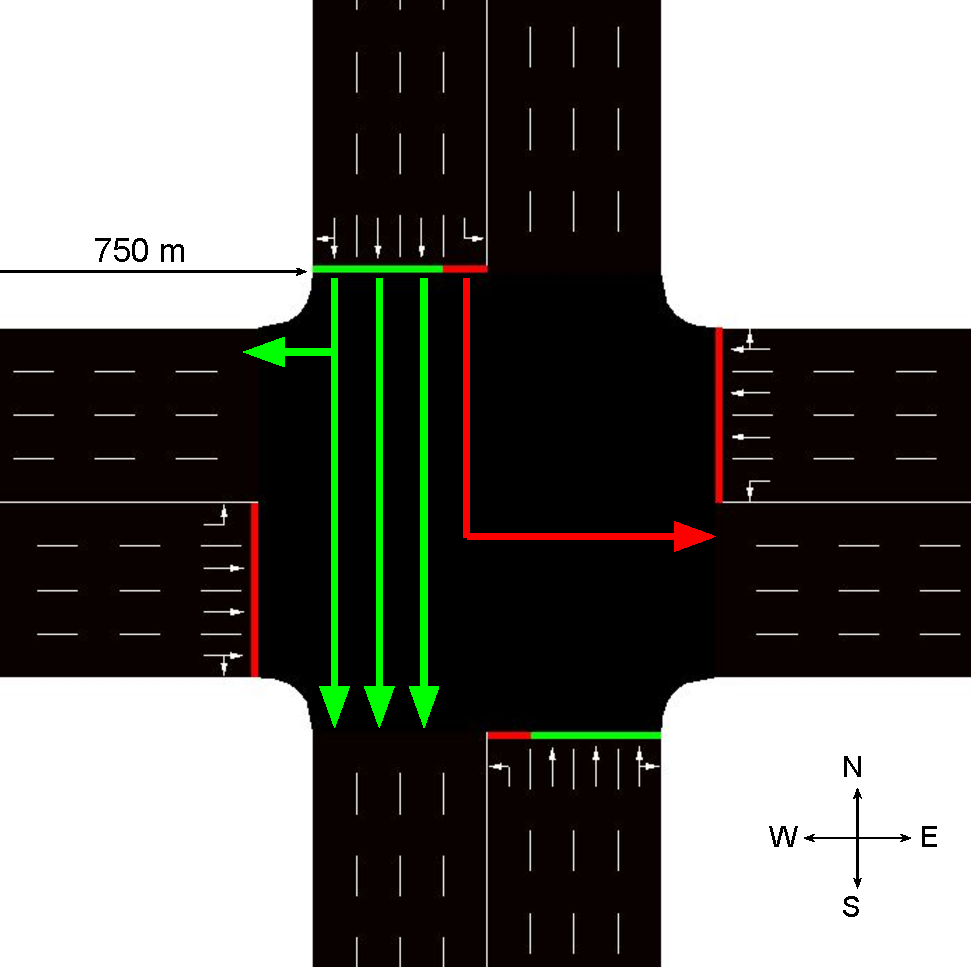
\includegraphics[scale=0.5]{images/Intersection.pdf}
    \end{center}
    \caption{A four-road intersection environment.}
    \label{fig:1}
\end{figure}

The traffic light (our agent) has a goal to maximize a special metric to evaluate its efficiency. Based on our assumption we can formulate our problem as following: given a state of intersection, and in order to maximize the efficiency; the agent has to select from a specified set of actions. In short, to formulate the traffic light signal control problem based on reinforcement learning, system state, actions, the reward function, and the agent learning approach should be defined. 

\begin{figure}[ht]
    \centering
    \begin{center}
    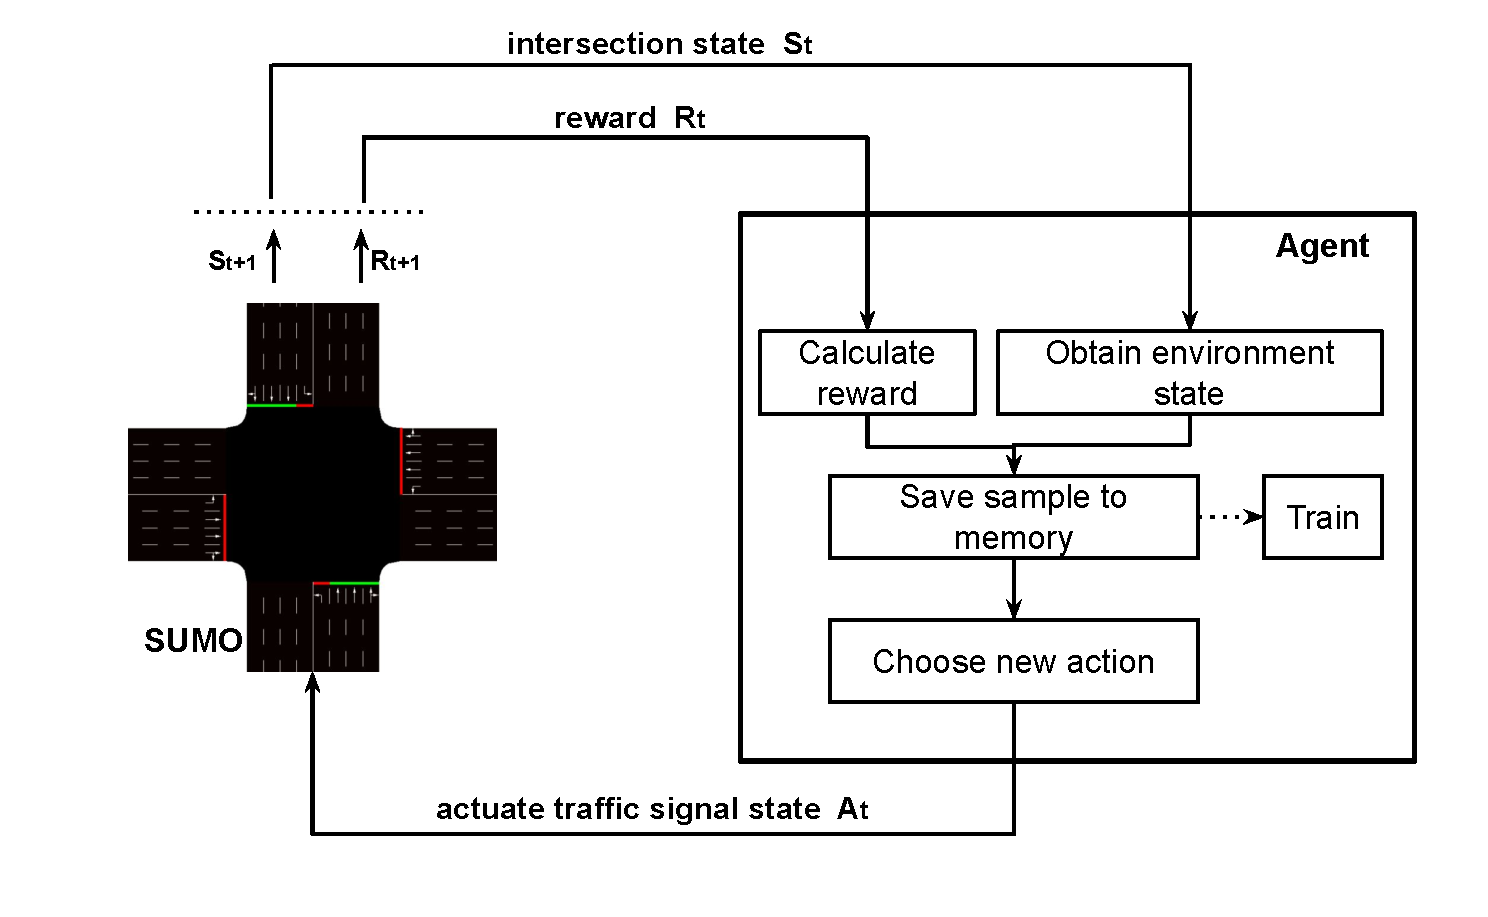
\includegraphics[scale=0.35]{images/RL_TSC_Scheme.pdf}
    \end{center}
    \caption{Reinforcement learning agent for traffic signal control.}
    \label{fig:2}
\end{figure}

The formulation of the problem and the general workflow of the agent can be shown in Fig.~\ref{fig:2}, where the agent interacts with the environment in discrete time steps, $t = 0, 1, 2, \cdots$. It should be highlighted that steps in the SUMO simulation represent time passing, which we will call "steps". The agent only functions at specific time steps, which we will refer to as "agentstep". As a result, the agent begins to acquire the current intersection state $S_{t}$ of the environment after many simulation steps. The action $A_{t}$ is selected and this action transitions the intersection state to the next state $S_{t+1}$ as vehicles move under the actuated traffic signal. Furthermore, the agent uses some indicators of the current traffic situation to determine the reward $R_{t}$ for the previous action actuated. Moreover, a memory is used to store the sample of data comprising all of the details of the most recent simulation steps, which is then afterwards retrieved for a training session. Hence, the sequence of the agent's interaction with the environment can be described as $\cdots, S_{t}, A_{t}, R_{t}, S_{t+1}, \cdots$. The following step is to specify the intersection state $S_{t}$, agent action $A_{t}$, and reward $R_{t}$. 

\subsection{Environment State}

The state $S_{t}$ is a model of the environment at a specific agentstep $t$. We need to give the agent enough information abot its environment and how the vehicle are distributed on each lane in order to make the agent learn how to optimize the traffic flow. In literature, the road lanes were discretized to set of cells and expressed as a vector that marking a cell with a 1 if a vehicle is present there and a 0 otherwise \cite{state}. In \cite{Adaptive}, a new vector represent the velocity of the vehicles is combined with position vector. A third vector is added by \cite{genders2016using} that represents the traffic light phase. 

The selected representation's aim, which was inspired by the discrete traffic state encoding (DTSE) \cite{genders2016using}, is to inform the agent at agentstep $t$ about the location of cars inside the environment.
More specifically, the adopted state design is irregular in shape and contains only spatial data about the cars placed within the environment. The discretization of the continuous environment is done using irregular cells. The incoming lanes on each road of the intersection are technically divided into small areas that can determine whether or not a vehicle is present.

Fig.~\ref{fig:3} shows the state representation for an intersection's road proposed by \cite{Deep}, where there are 20 cells between the start of the route and the stop line at the intersection. Half of the cells are assigned along the left-only lane, while the other half is spread out over the other lanes. Each cell's size varies according to its distance from the end line; the bigger the area, the more distance - from the lane - it covers. Each cell's length must be carefully chosen. The smallest areas, which are also the nearest to the end line, are bigger than the car's size. 

Since there are 80 cells total in the 4-road intersection, The presence or absence of vehicles in each cell will be described by the agent observation of the environment state.

\begin{figure}[H]
    \centering
    \begin{center}
    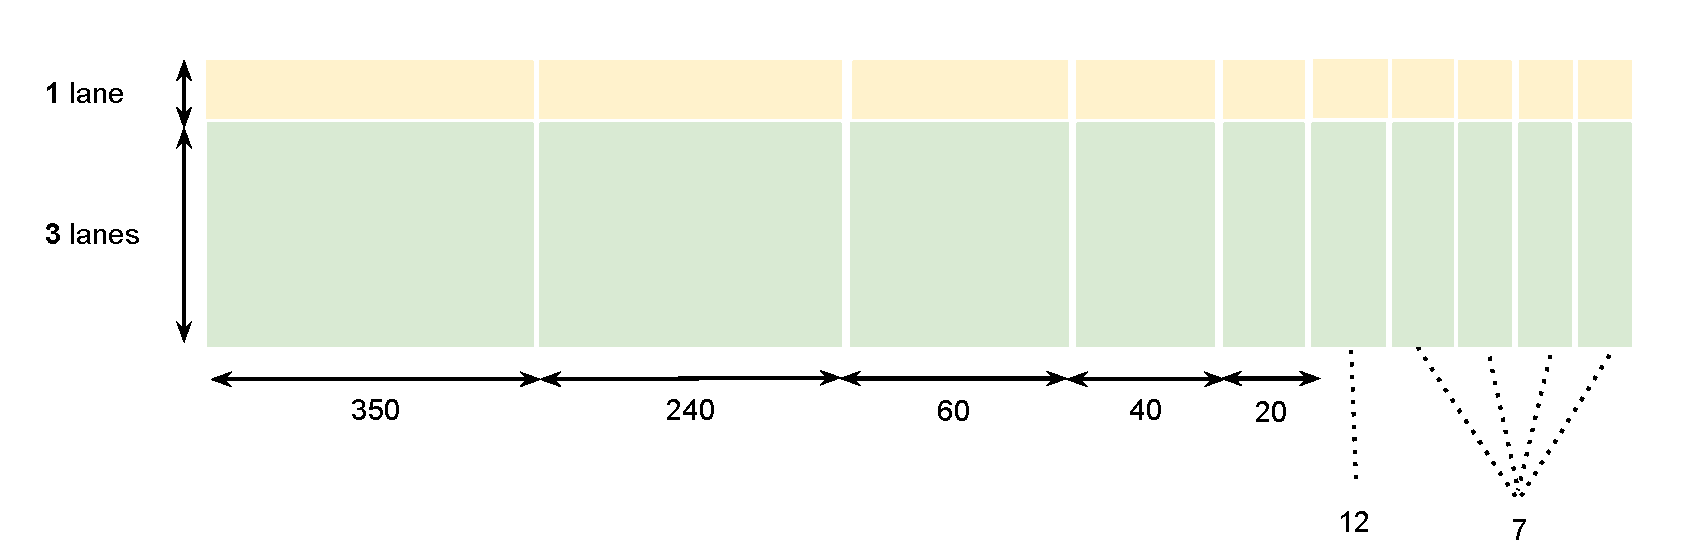
\includegraphics[scale=0.31]{images/State cells length.pdf}
    \end{center}
    \caption{State representation design with cells length.}
    \label{fig:3}
\end{figure}

\subsection{Agent Action Set}

Because the agent is a traffic light system, so doing an action means activating the green stage of a set of lanes for period of time. We defined he green duration as a 10 seconds, while the yellow duration is defined as 4 seconds. The actions represents all of the possible choices that the agent can take. (\ref{Eq:1}).

\begin{equation}\label{Eq:1}
    A = \{NS, EW, NSL, EWL\}
\end{equation}

The following is a description of every action in set (\ref{Eq:1}).

\begin{itemize}
    \item North-South (NS): Vehicles on the north and south roads are allowed to go straight ahead or make a right turn during the green period.
    \item East-West (EW): Vehicles on the east and west roads are allowed to go straight ahead or make a right turn during the green period.
    \item  North-South Left (NSL): During the green period, vehicles in the specified sides are permitted to turn left.
    \item  East-West Left (EWL): During the green period, vehicles on the east and west roads are permitted to turn left.
\end{itemize}\leavevmode\\

The four potential actions are represented graphically in Fig.~\ref{fig:4}.

\begin{figure}[H]
    \centering
    \begin{center}
    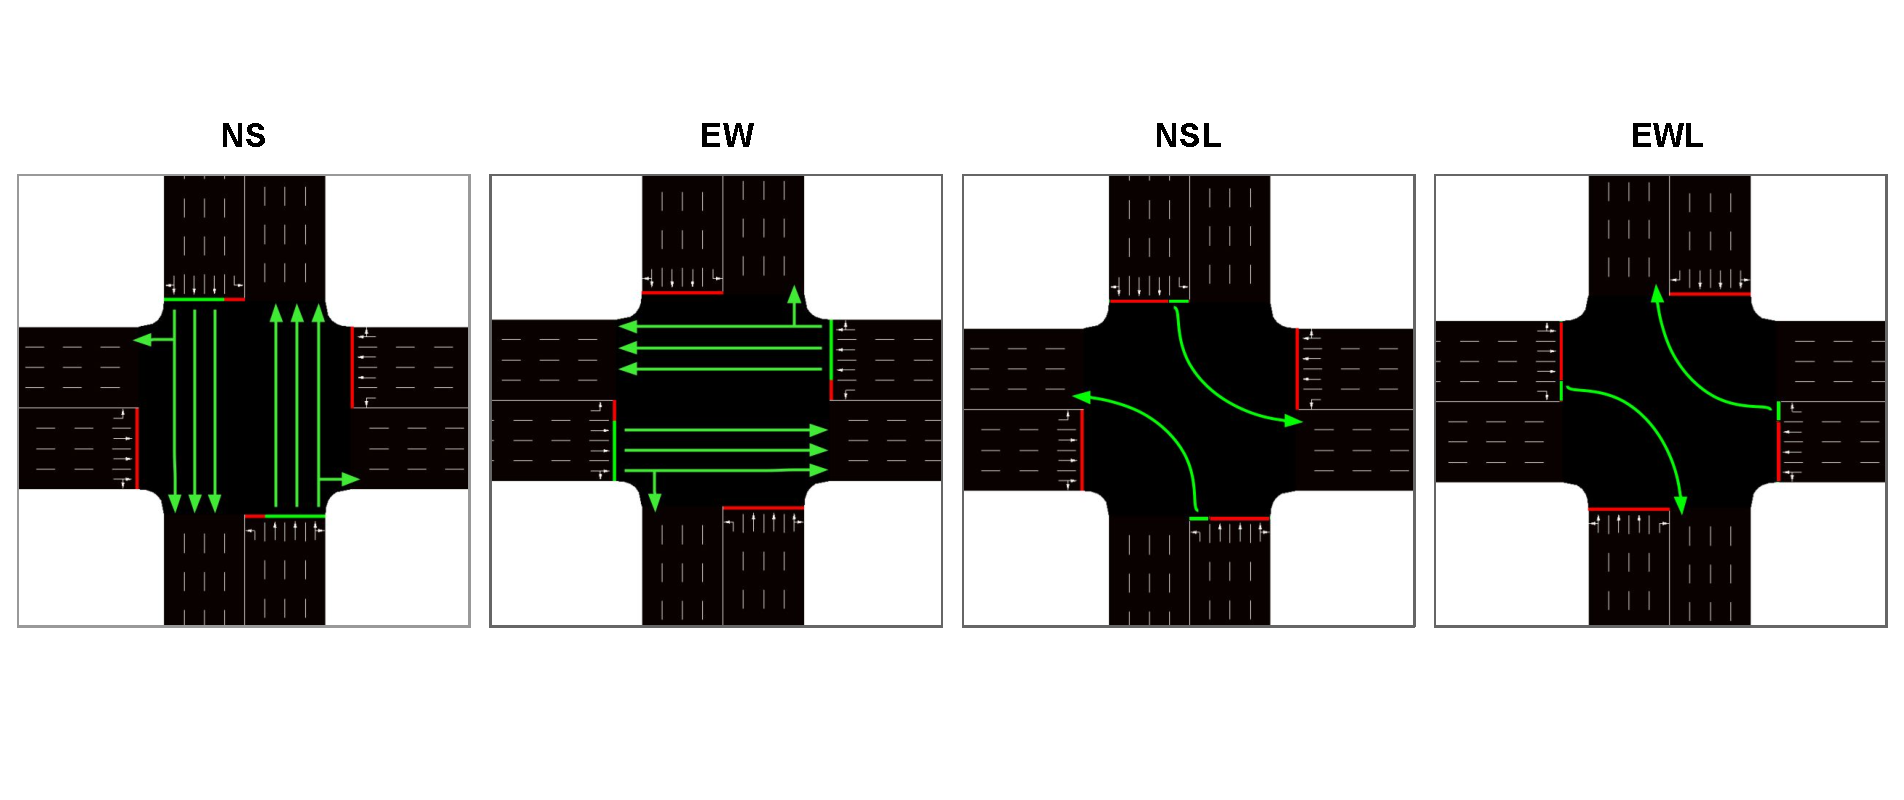
\includegraphics[scale=0.27]{images/Possible actions.pdf}
    \end{center}
    \caption{The graphical representation of the four potential actions.}
    \label{fig:4}
\end{figure}

We should mention that if the state of the traffic light did not change, then the yellow sign wont be activated. But if we have a situation where the action is changed, then a yellow phase will start with 4 seconds simulation time and we will have a total simulation time between a two actions is 14 seconds (yellow phase in addition to the green phase). This process outline is depicted in Fig.~\ref{fig:5}, where first choosing the same action (NS), then translating from Action (NS) to Action (NSL).

\begin{figure}[H]
    \centering
    \begin{center}
    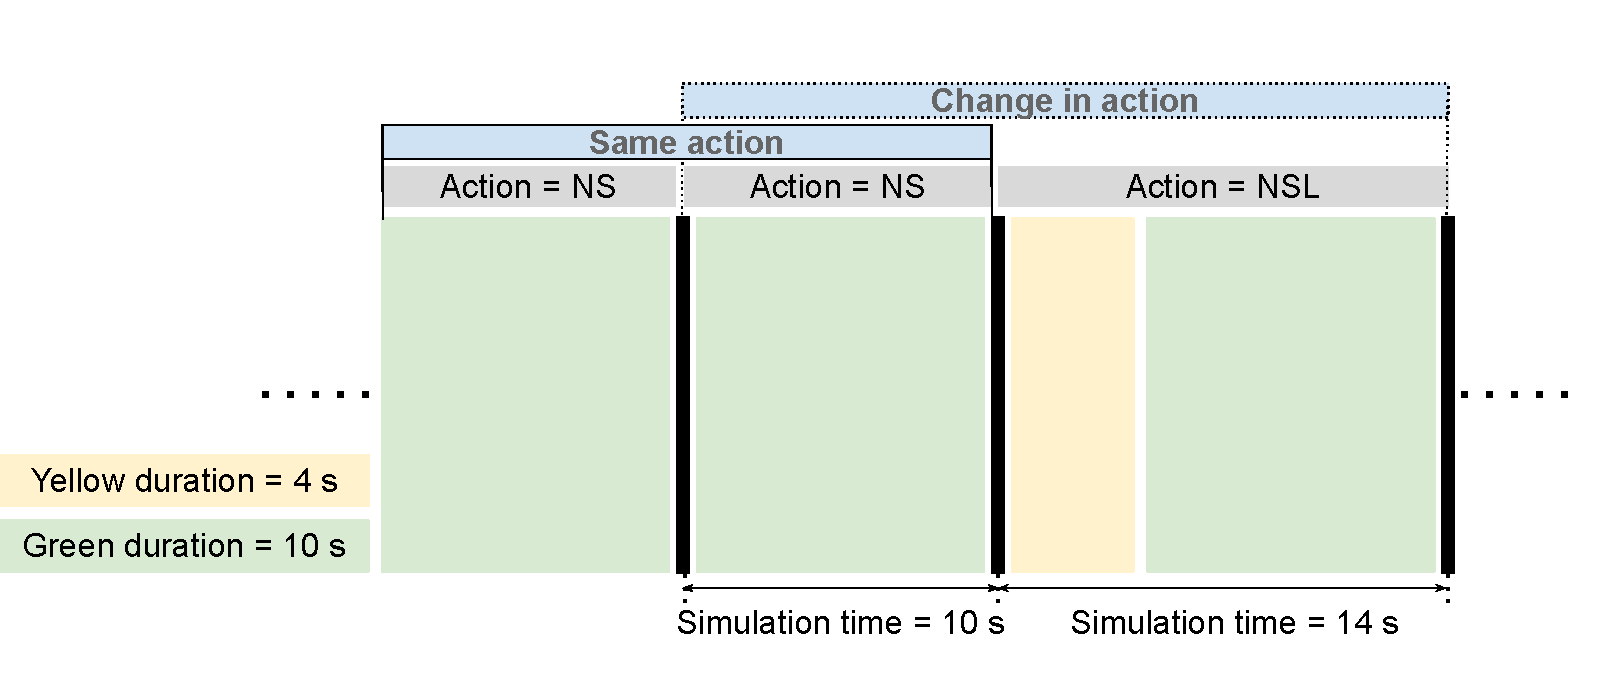
\includegraphics[scale=0.3]{images/Simulation steps.pdf}
    \end{center}
    \caption{Possible simulation time of chosen actions.}
    \label{fig:5}
\end{figure}

It should be noted that in a real-world application, such a presented agent can be easily replaced with a traffic control system. 

\subsection{Reward Function}
The agent must evaluate and comprehend the chosen action's efficacy in the most recent state to improve the way of choosing the future actions. The reward function, like vehicle delays, queue lengths, and waiting times, is a performance efficiency indicator \cite{Deep}. The cumulative waiting time of each vehicle, which leads to a cumulative reward function is the most commonly used approach in the traffic congestion problem, as adopted in \cite{genders2016using} and \cite{Deep}. In literature a weighted sum of multiple indicators combined together as suggested in \cite{Intellilight}. To summarize, reward is the agent's way of evaluating the action he has taken, allowing him to improve his model of choices later on. 

We can write the reward function however we want. In our problem, our goal is to reduce vehicle waiting time at traffic lights, but we want to cast it as a maximization problem, As a result, our goal is to gradually increase traffic flow through the intersection. To accomplish this in a realistic manner, the reward obtained from calculating the mean of the delay and travel time. Therefore, the agent must be aware of whether the decision he takes makes him close or far away from the desired goal (increasing traffic flow through the intersection). 

The reward function varies depending on the performance measures that are considered. So, we will present two different reward function: Literature reward function and Alternative reward function.

\begin{enumerate}
    \item [1)] Literature reward function:
    This function is named after studies that addressed the same problem, and uses the total waiting time as a metric as formulated in Eq.~\ref{Eq:2} where $twt t$ is the total waiting time in agentsetep $t$ and $n$ is the number of vehicles in the queue.
    \begin{equation}
    \label{Eq:2}
    twt_t= \sum_{veh=1}^{n} {wt_{veh,t}}
    \end{equation}
    
    Hence, the literature reward function can be formulated as follows.
    \begin{equation}
    \label{Eq:3}
    r_t= twt_{t-1} - twt_t
    \end{equation}
    
    From Eq.~\ref{Eq:3}, a negative reward is associated with a bad action that increases the number of vehicles in queues in the current agentstep $t$ relative to the condition in the prior agentstep $t-1$, leading to wait for more time than in the previous agentstep. \cite{Deep}.\\
    
    \item [2)] Alternative reward function:
    This function differs from the previous function in the metric as it uses the \textit{accumulated waiting time} defined in Eq.~(\ref{Eq:4})
    \begin{equation}
    \label{Eq:4}
    atwt_t= \sum_{veh=1}^{n} {awt_{veh,t}}
    \end{equation}
    
    Thus, the alternative reward function can be defined as follows.
    \begin{equation}
    \label{Eq:5}
    r_t= atwt_{t-1} - atwt_t
    \end{equation}
    
    $atwt t$ is the total amount of waiting time. By using this reward function, we can ensure that when the vehicle departs but is unable move forward (after intersection), $atwt t$ doesn't reset, to avoid the case  when a long queue appears at the intersection, as well described in \cite{Deep}.

\end{enumerate}


\subsection{Agent Goal}
The main goal in our case is to increase traffic flow through the intersection by reducing the vehicles waiting time. The agent observation of the intersection state, the agent must choose the appropriate action, which will be in accordance with action policy $\pi^*$. Each time step will have a reward for each action ($R_{t}, R_{t+1}, R_{t+2}, \cdots$). We must emphasize a critical point here: when formulating our problem, we must define the agent's goal with respect to time: Do we need to achieve this goal one time? More formally, the agent should find an optimal policy $\pi^*$ that maximizes the to be predicated cumulative reward is described by the action-value function in Eq.~\ref{Eq:6}.
\begin{equation}
    \label{Eq:6}
    Q_{\pi}(s,a) = \mathop{\mathbb{E}}\{ R_t+\gamma R_{t+1} + \gamma^2R_{t+2}+...|S_t=s,A_t=a,\pi\}
\end{equation}
\begin{equation*}
    = \mathop{\mathbb{E}}\{\sum_{k=0}^{\infty}\gamma^kR_{t+k}|S_t=s,A_t=a,\pi\}
\end{equation*}
where $\gamma$ is a discount factor, $0\leq\gamma\leq1$, so when $\gamma=0$ indicates the immediate reward only, and when $\gamma$ reaches $1$ ithe agent is more foresighted.

Such an optimal policy $\pi^*$ can be given by
\begin{equation}
    \label{Eq:7}
    \pi^*= \underset{\pi}{\operatorname{argmax}} Q_\pi(s,a) \quad for \quad all \quad s\in S, a \in A
\end{equation}


\section{Deep Q-Learning Algorithm}\label{DNN}

We introduce here the deep Q-Learning algorithm, which consists of deep neural networks and Q-Learning\cite{Q-learning}. To achieve the agent goal (finding the optimal action policy $\pi^*$), the optimal Q-values $Q^*(s,a)$ are required to be obtained. As if the optimal Q-values $Q^*(s,a)$ for all pairs of state-action are known, the agent can find the optimal action policy $\pi^*$ by basically picking the action $a$ that results in the optimal Q-values $Q^*(s,a)$ for a state $s$. The optimal Q-values $Q^*(s,a)$ can be calculated from Bellman optimality recursive equation\cite{RL-Intro} as follows. 

\begin{equation}
\label{Eq:8}
\begin{aligned}
     Q^*(s, a)=\mathbb{\mathbb{E}}\{R_t+\gamma \underset{a^{\prime}}{\operatorname{max}}Q^*(S_{t+1}, a^{\prime})| S_t=s, A_t=a\} \\
    \quad for \quad all \quad s\in S, a \in A
\end{aligned}
\end{equation}

If the total number of states is finite and we are aware of every aspect of the underlying system model, such as the transition probabilities of intersecting states and related expected reward, we can theoretically solve the Bellman optimality equation \ref{Eq:8} to obtain the optimal Q-values $Q^*(s,a)$. Since the traffic environment is dynamically changing at the intersection, it is impossible to find the transition probabilities for the large intersection states caused by complex traffic scenarios. Therefore, Q-Learning has been widely utilized to overcome these issues, as it is a model-free\cite{watkins1989learning} reinforcement learning approach where there is no need for these transition probabilities. The action value function $Q\left(s_t, a_t\right)$ of picking action $a_t$ at state $s_t$ is defined as follows.


\begin{equation}
   \label{Eq:9}
   Q(S_{t},a_{t})= Q(S_{t},a_{t})+\alpha(r_{t+1}+\gamma \cdot \max_{A}Q(s_{t+1},a_{t})-Q(s_{t},a_{t}))
\end{equation}

This equation updates the Q-value by learning rate $\alpha$ that discounts the updated quantity. The temporal link between doing the action $a_t$ and getting the resultant reward is highlighted by the subscript $t+1$. So, the reward for moving from state $s_t$ in to state $s_{t+1}$ taking an action $a_t$ is represented by $r_{t+1}$. The expression $max _A$ denotes that the most valuable action is chosen of all those available in the state $s_{t+1}$. 

Authors in \cite{Deep} used a modified version of Eq.~\ref{Eq:10} to calculate the Q-Learning function as follows.
\begin{equation}
   \label{Eq:10}
   Q(S_{t},a_{t})= r_{t+1}+\gamma \cdot \max_{A}Q^{\prime}(s_{t+1},a_{t+1})
\end{equation}

where the Q-value for the action $a_{t+1}$ in the state $s_{t+1}$, or the state that comes after taking an action $a_{t}$ in the state $s_{t}$, is referred to as $Q^{\prime}(s_{t+1},a_{t+1})$. 

It is frequently unfeasible to find and save each state-action pair in a reinforcement learning application due to the large state space. As a result, a deep neural network (DNN) is used to approximate the Q-learning function that results in $Q(s, a) ≈ Q^*(s, a)$.

\subsection{Deep Neural Network Architecture}
In this study, a fully connected DNN is used as graphically presented in Fig.~\ref{fig:6}. The input layer has 80 neurons which represents the total number of cells at the intersection state. The input layer is then followed by 5 hidden layers, 400 neurons each, and activated using (ReLU) function \cite{ReLU}. The output layer consists of four neurons corresponding to the 4 possible action values with a linear activation function. 

\begin{figure}[!ht]
    \centering
    \begin{center}
    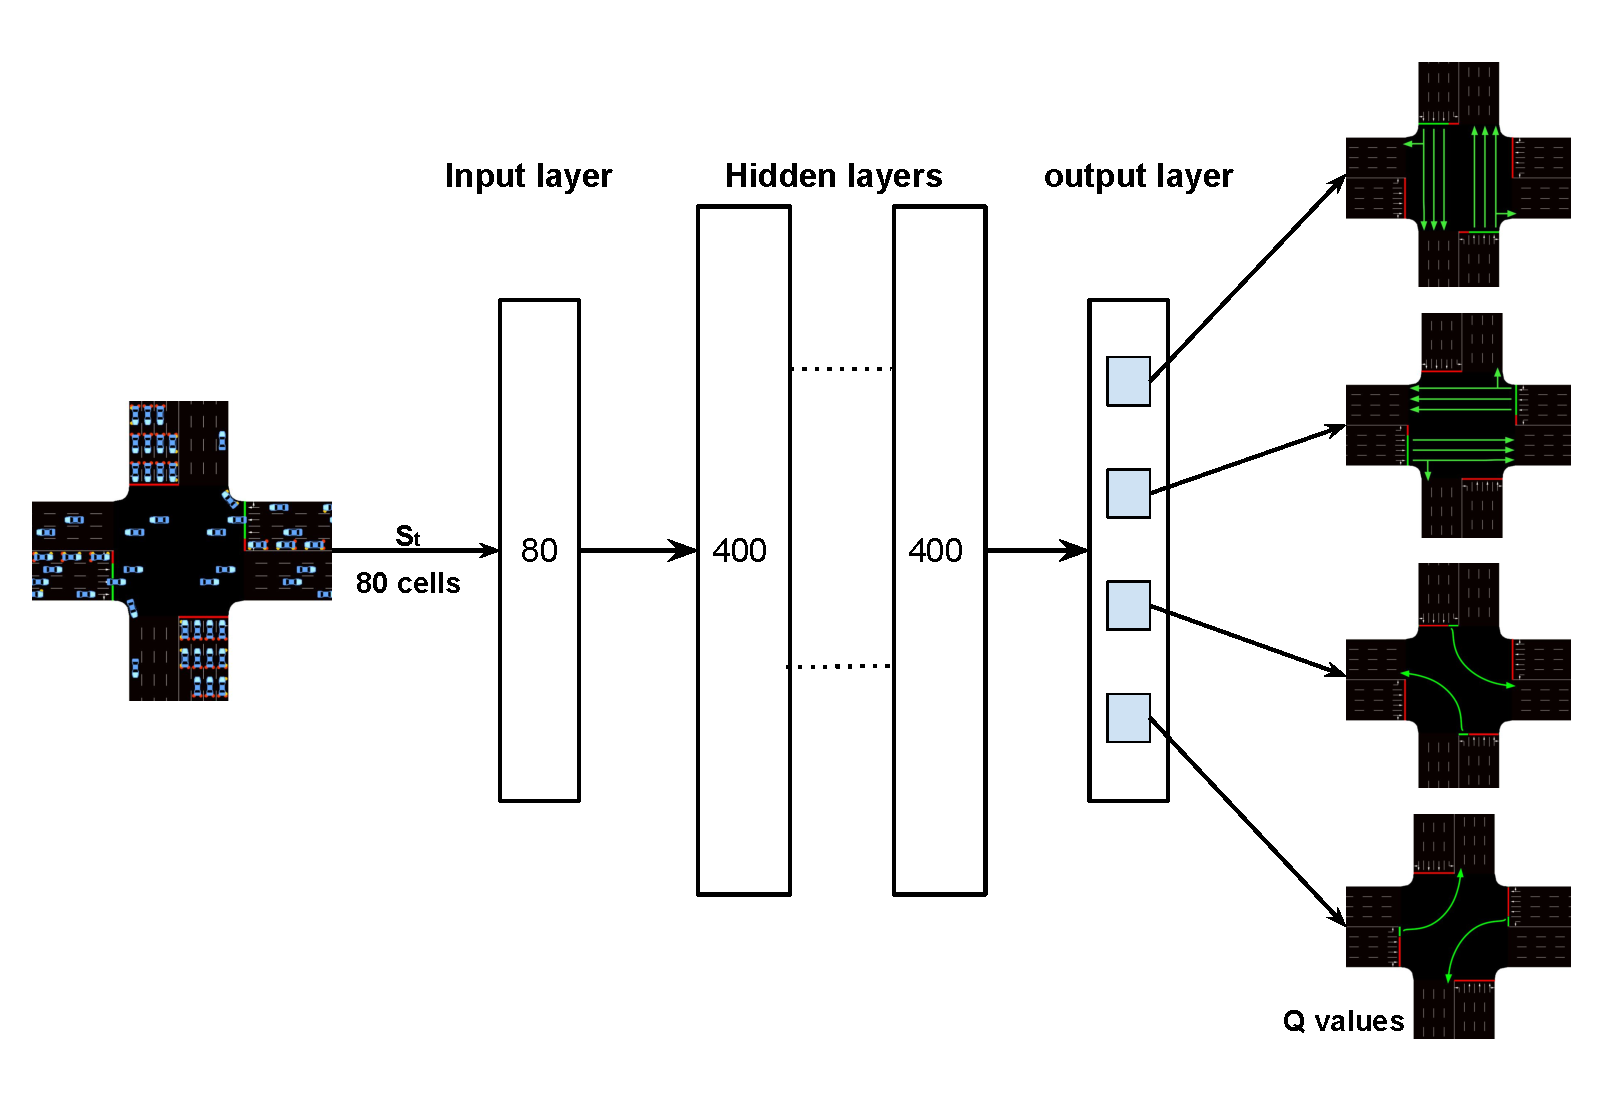
\includegraphics[scale=0.3]{images/DNN.pdf}
    \end{center}
    \caption{Deep neural network architecture.}
    \label{fig:6}
\end{figure}

To enhance the agent's performance and learning effectiveness during the training, experience replay\cite{replay} technique is implemented. Instead of giving the agent the data it learns throughout the simulation right away, this method involves giving it the information it needs to learn in the form of a batch of randomly selected samples (commonly called Online Learning). Since the environment's state $s_{t+1}$ is the next state of $s_t$ and the agent will be learnt more in $S_{t+1}$, so the correlation might reduce the agent's capacity to learn, this approach is used to eliminate correlations in the observation sequence. The scheme of data collection task is depicted in Fig.~\ref{fig:7}.

\begin{figure}[!ht]
    \centering
    \begin{center}
    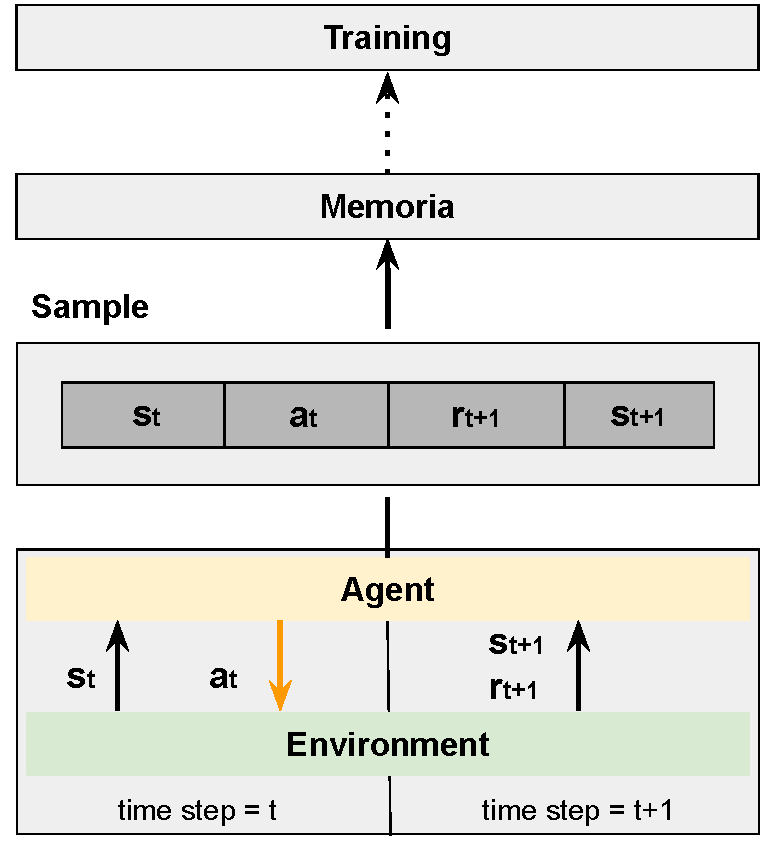
\includegraphics[scale=0.4]{images/Data_collection.pdf}
    \end{center}
    \caption{Data collection task.}
    \label{fig:7}
\end{figure}

As shown in the above scheme, each sample ($E$) can be formed by the set (\ref{Eq:11}).

\begin{equation}\label{Eq:11}
    E_t = \{S_{t}, A_{t}, R_{t+1}, S_{t+1}\}
\end{equation}

The batch is drawn from a data structure known as memory ($M$), which holds each sample collected throughout the training phase. 
\begin{equation}\label{Eq:12}
    M = \{E_{t}, E_{t+1}, E_{t+2}, \cdots\}
\end{equation}

It is defined by a memory size and a batch size. In this model, the memory size was set to 5000 which represents the maximum number of samples that memory can hold. The memory size, which is set at 50000 samples, indicates how many samples the memory can hold. The batch size is set to 100 and it indicates the quantity of samples that are brought from memory during one training occurrence. 

\subsection{Deep Neural Network Process}
The training process is performed iteratively for each training instance using the extracted data from the batch samples. Fig.~\ref{fig:8} shows the training procedures that are carried out from the perspective of each sample.

\begin{figure}[!ht]
    \centering
    \begin{center}
    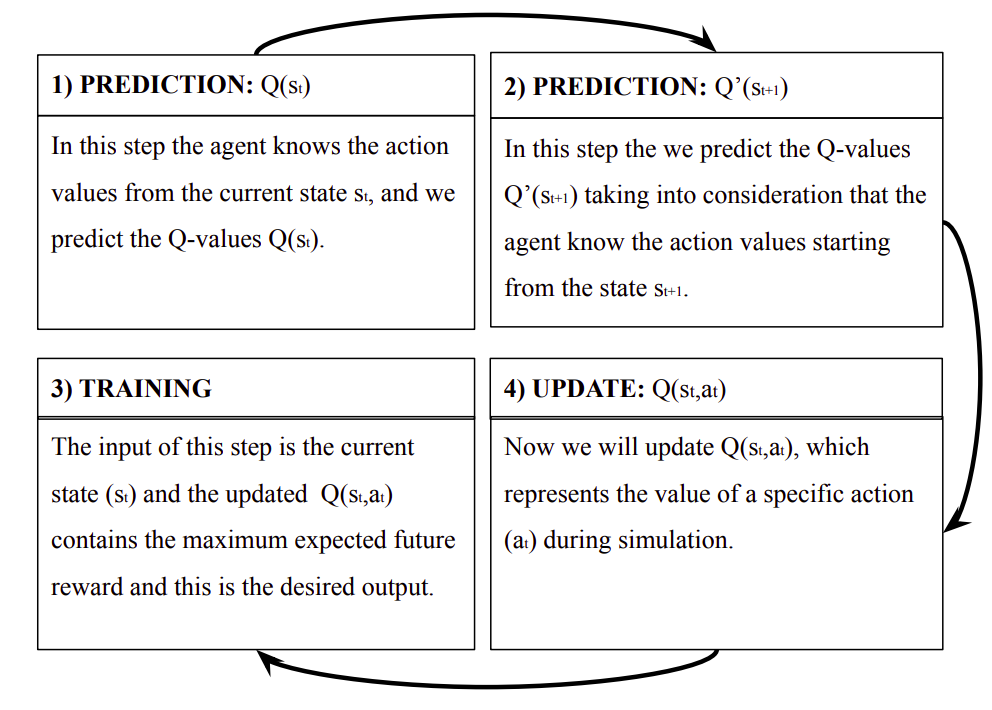
\includegraphics[scale=0.25]{images/Training_Process.png}
    \end{center}
    \caption{Training process scheme.}
    \label{fig:8}
\end{figure}

It should be noted that during the update of $Q(s, a)$, the greedy method is adopted to choose the action that maximizes the predicted action value function $Q^{\prime}(s_{t+1},a_{t+1})$ as described in Eq.~\ref{Eq:10}. However, this is not always the case when performing. We use the $\epsilon-greedy$ policy, described in Eq.~\ref{Eq:13}, which performs the exploration with probability $\epsilon$ and chooses the exploitation with probability $1-\epsilon$. 

\begin{equation}\label{Eq:13}
    \epsilon_{n} = 1 - \frac{n}{N}
\end{equation}

where $n$:current episode $N$:total number of episodes. Initially, $\epsilon$ is set to 1, indicating that the agent only explores. But as the training progresses, $\epsilon$ gradually decreases, allowing the agent to exploit what it has learned more and more exclusively. 

Once the DNN has approximated the Q-Learning function, the optimal policy $\pi^*$ is obtained, which selects the highest action value given the current state to maximize traffic efficiency.

\section{Simulation Setting}\label{SS}

In this section, we will demonstrate the setup for the SUMO simulation. In addition, the traffic route generation approach will be presented.

\subsection{Training Setup}
As we are working with a simulator, it is important to start by calculating the training time. We set the duration for each episode to 2 hours,and SUMO's default time frequency is one second. Therefore, N is 7200. To project this on a real life scenario, we set 100 episodes of 2 hours each, which is more than eight days of nonstop traffic, and by using a high-graphics laptop we managed to finish the entire training by 3.5 hours. 

\subsection{Traffic Route Generation}
Traffic generation is a very critical point in our problem and to maintain a high level of realism, we used a Weibull distribution (shape = 2) to as it was proposed by \cite{Deep}.
The distribution is represented as a histogram, with the number of vehicles generated on the Y-axis and the steps of one episode on the X-axis. The Weibull distribution, as discussed in \cite{Deep} where cars number increases early on, representing the busiest hour in the day and this simulates a real-life situations. The number of arriving cars then gradually decreases, as shown in Fig.~\ref{fig:9}. Furthermore, the dimensions and performance of each generated vehicle are the same.

\begin{figure}[!ht]
    \centering
    \begin{center}
    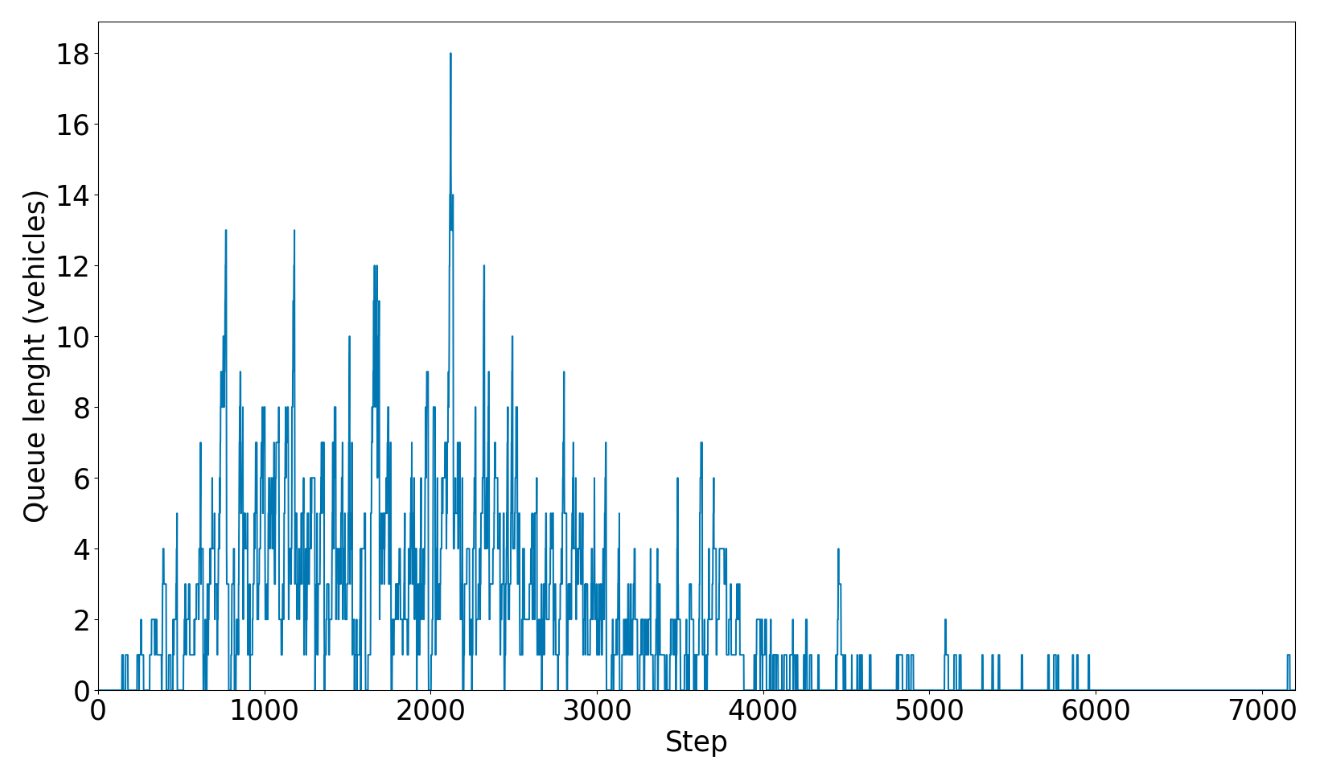
\includegraphics[scale=0.25]{images/weibull.png}
    \end{center}
    \caption{Weibull distribution for traffic generation on a single episode.}
    \label{fig:9}
\end{figure}

To get an adaptive agent, we should include different scenarios as follows.
\begin{enumerate}
    \item [-] High traffic scenario: four thousands cars reach the intersection.
    \item [-] North-South (NS) traffic scenario: The traffic in this scenario is neither high nor low; it is in the middle, with two thousands cars arriving at the intersection.
    \item [-] East-West (EW) West traffic scenario: The traffic in this scenario is neither high nor low; it is in the middle, with two thousands cars arriving at the intersection.
    \item [-] Low traffic scenario: six hundred cars arrive at the intersection.
    
\end{enumerate}
Each episode will represent different scenario, and scenarios will iterate throughout the training.


\section{Simulation Results}\label{SR}

The agent performance is examined using the training's reward trend followed by some metrics. These metrics evaluate the behavior of the traffic light system (agent) behaviour. The metrics used are the average queue length (number of vehicles) and the cumulative delay time for all vehicles at the intersection. Fig.~\ref{fig:10} illustrates how agent's learning progressed throughout training in terms of cumulative negative reward. As can be shown, the agent has acquired a sufficiently correct policy. 

\begin{figure}[!ht]
    \centering
    \begin{center}
    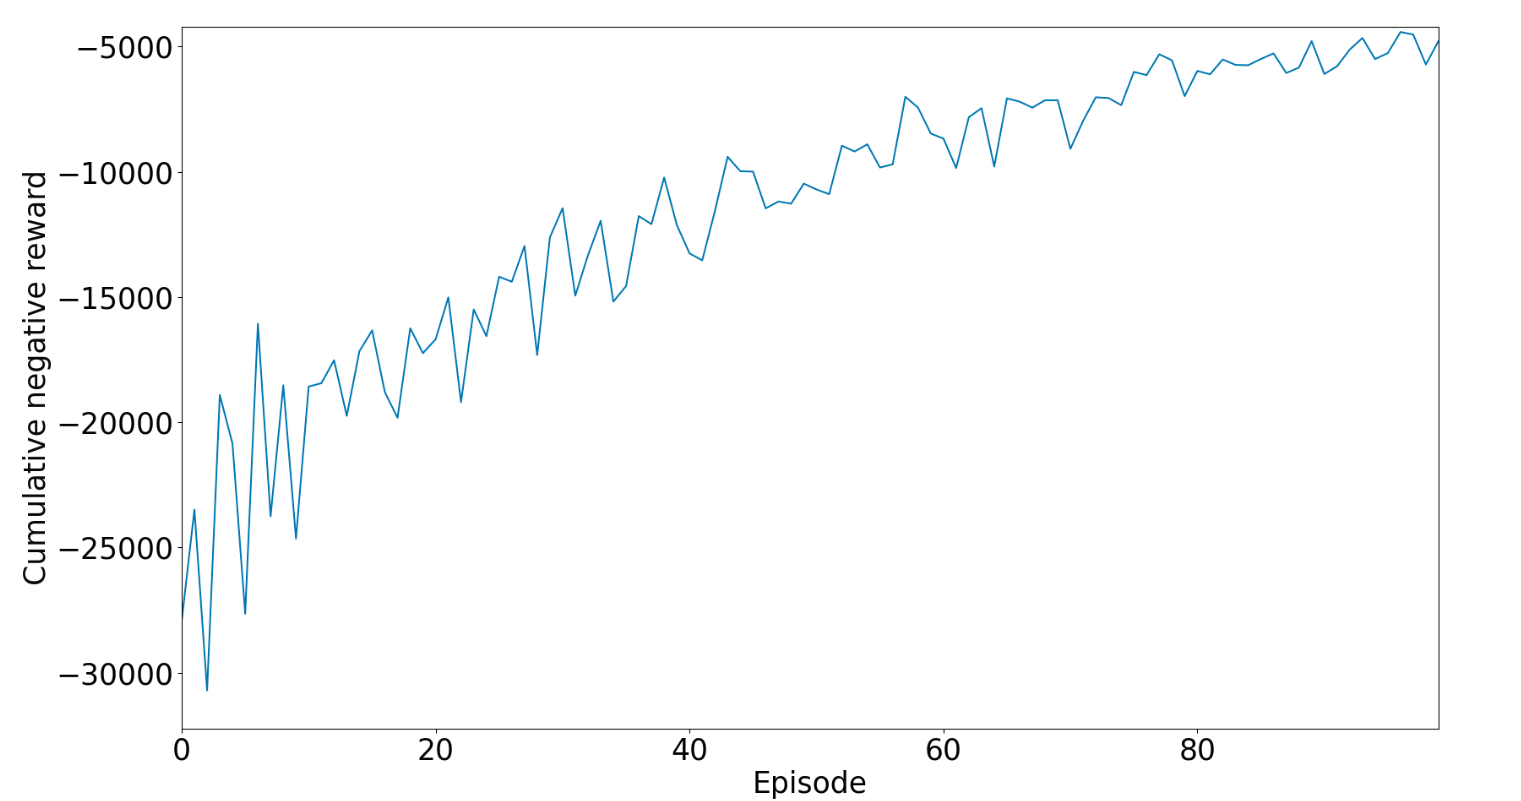
\includegraphics[scale=0.23]{images/train_reward.png}
    \end{center}
    \caption{Cumulative negative reward during the training per episode.}
    \label{fig:10}
\end{figure}

The total accumulative waiting time (delay) was measured during the training using the alternative reward function which accumulates each waiting time for the vehicle until it passes the intersection. This function has proven its efficiency especially in long queues as it does not reset vehicles' waiting times by any simple movement through the queue. Fig.~\ref{fig:11} shows the accumulative delay time during the training episodes. At the end of training, the agent managed to reduce the waiting time by utilizing the learned policy which is obtained by an appropriate approximation of the Q-values. 

\begin{figure}[!ht]
    \centering
    \begin{center}
    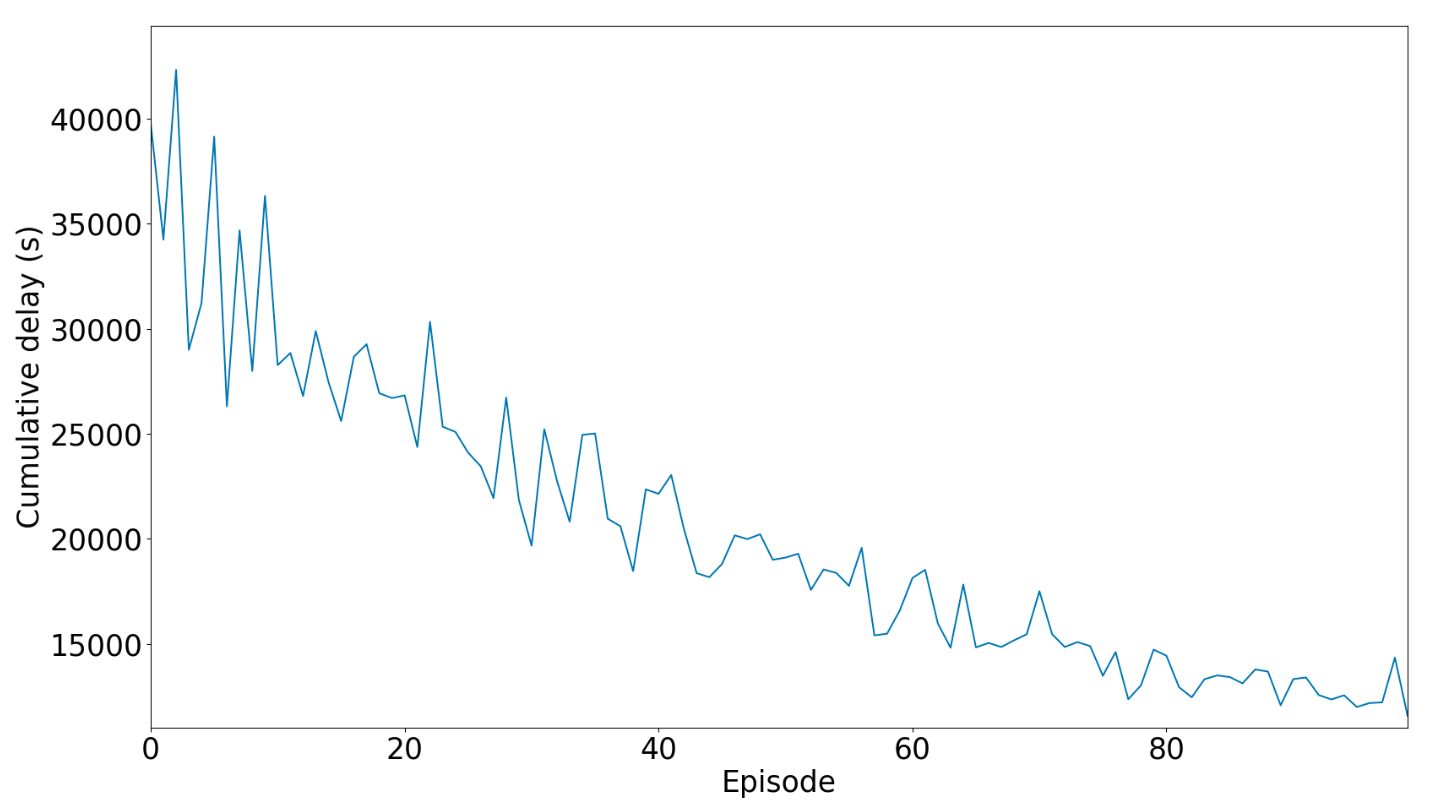
\includegraphics[scale=0.24]{images/train_delay.png}
    \end{center}
    \caption{Cumulative delay during the training per episode.}
    \label{fig:11}
\end{figure}


\begin{figure}[!ht]
    \centering
    \begin{center}
    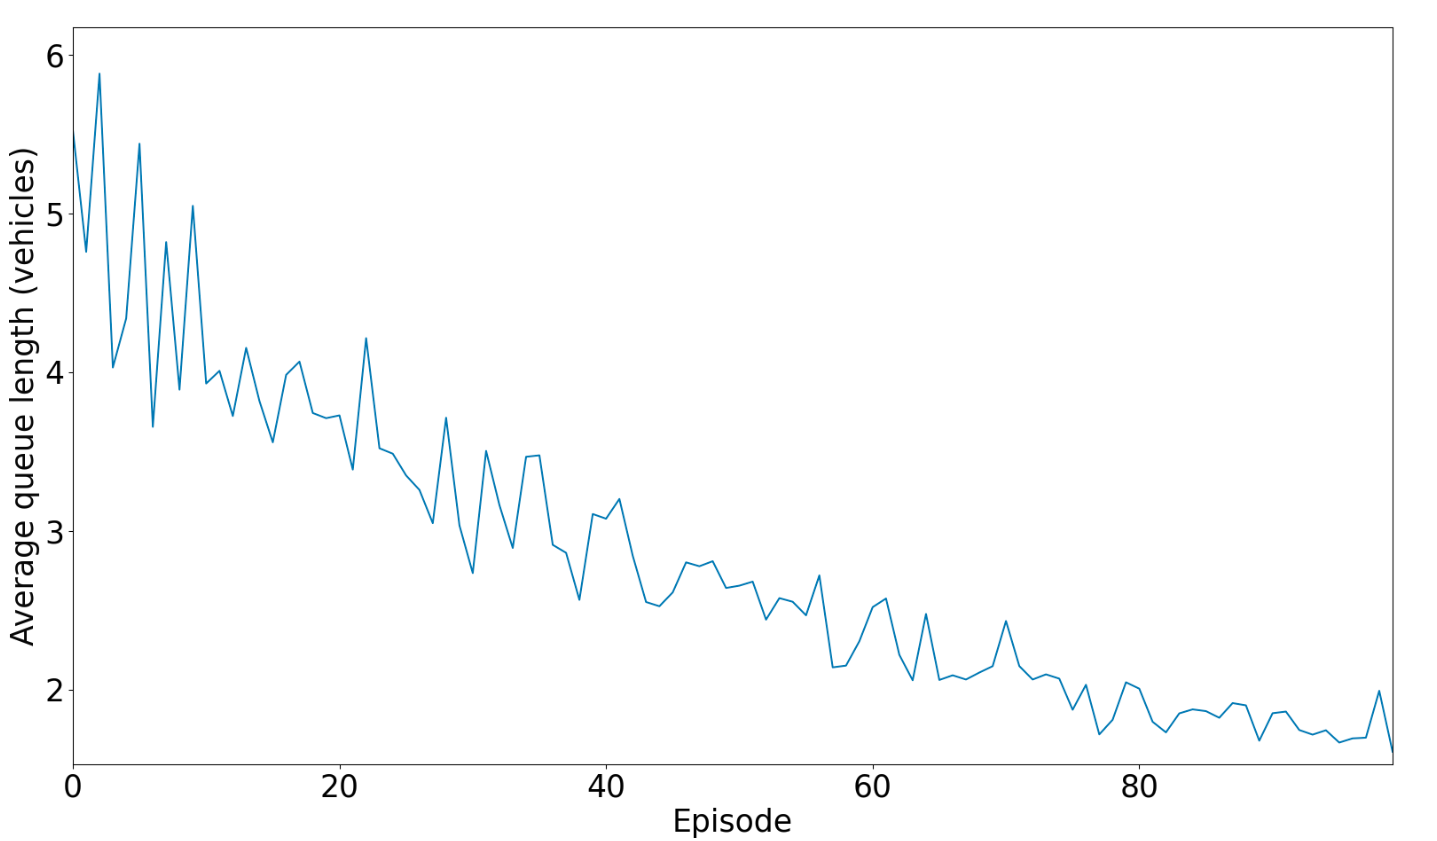
\includegraphics[scale=0.24]{images/train_queue.png}
    \end{center}
    \caption{Average queue length during the training per episode.}
    \label{fig:12}
\end{figure}

The corresponding metric for the cumulative waiting time is the queue length, which indicates the average number of cars queued per step in each episode. Fig.~\ref{fig:12} represents the average queue length (vehicles) through the training episodes. 

Model testing is performed and the associated reward to the actions taken at the agentstep is recorded as depcited in Fig.~\ref{fig:13}. It is noticeable that there are some negative rewards at some agentstep which indicates that the agent has chosen a bad action. However, the agent still perform well as the number of the good actions dominates the one of the bad actions which can be interpreted by the the reward values as shown in Fig.~\ref{fig:13}.

\begin{figure}[H]
    \centering
    \begin{center}
    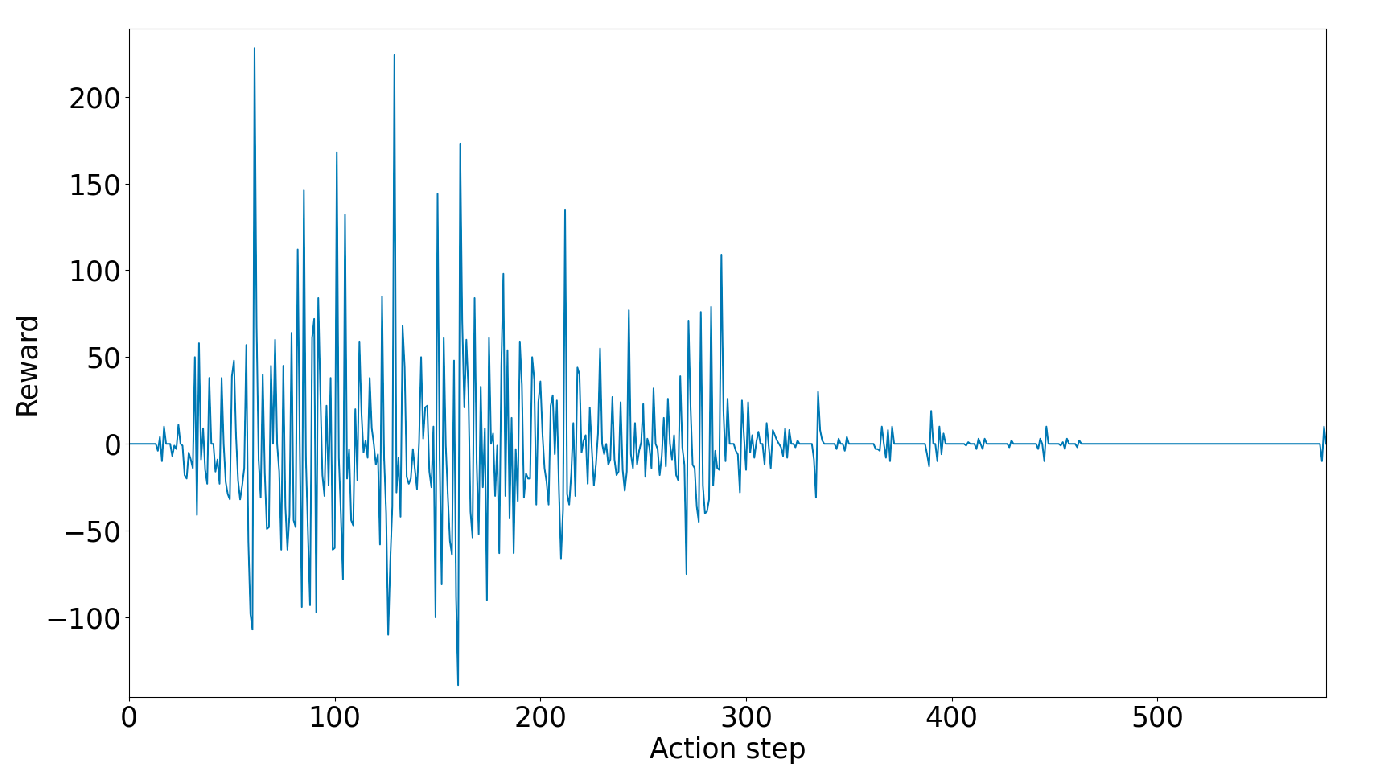
\includegraphics[scale=0.24]{images/test_reward.png}
    \end{center}
    \caption{Average queue length during the training per episode.}
    \label{fig:13}
\end{figure}

% after 100 of training episodes, the agent was able to ...

\section{conclusion}\label{Conclusion}
The paper presented a deep Q-Learning algorithm to overcome the traffic congestion problem. The proposed algorithm is based on a deep neural network that approximates the Q-learning function. Experience replay is coupled with Q-learning to eliminate the correlation in the observation sequence; consequently, improve the model performance. SUMO environment was generated to train and test the traffic light system (agent). Two metrics have been employed to evaluate the agent behaviour: the average queue length (numbers of vehicles), and the accumulative delay time for all vehicles at intersection. The results demonstrated that the proposed algorithm leads to a fair traffic control policy that maximizes traffic flow and reduces accumulative waiting time. 

Future work aims to improve the learning approach to accelerate convergence and avoid the occurrence of negative rewards. 

\bibliographystyle{IEEEtran}
\bibliography{Bibliography}

\end{document}






